\documentclass{article}
\usepackage{amsfonts, amsthm, amsmath, amssymb, mathtools, ulem, mathrsfs, physics, esint, siunitx, tikz-cd}
\usepackage{pdfpages, fullpage, color, microtype, cancel, textcomp, markdown, hyperref, graphicx}
\usepackage{enumitem}
\usepackage{algorithm}
\usepackage{algpseudocode}
\graphicspath{{./images/}}
\usepackage[english]{babel}
\usepackage[autostyle, english=american]{csquotes}
\MakeOuterQuote{"}
\usepackage{xparse}
\usepackage{tikz}

\usepackage{calligra}
\DeclareMathAlphabet{\mathcalligra}{T1}{calligra}{m}{n}
\DeclareFontShape{T1}{calligra}{m}{n}{<->s*[2.2]callig15}{}
\newcommand{\script}[1]{\ensuremath{\mathcalligra{#1}}}
\newcommand{\scr}{\script r}

% fonts
\def\mbb#1{\mathbb{#1}}
\def\mfk#1{\mathfrak{#1}}
\def\mbf#1{\mathbf{#1}}
\def\tbf#1{\textbf{#1}}

% common bold letters
\def\bP{\mbb{P}}
\def\bC{\mbb{C}}
\def\bH{\mbb{H}}
\def\bI{\mbb{I}}
\def\bR{\mbb{R}}
\def\bQ{\mbb{Q}}
\def\bZ{\mbb{Z}}
\def\bN{\mbb{N}}

% brackets
\newcommand{\br}[1]{\left(#1\right)}
\newcommand{\sbr}[1]{\left[#1\right]}
\newcommand{\brc}[1]{\left\{#1\right\}}
\newcommand{\lbr}[1]{\left\langle#1\right\rangle}

% vectors
\renewcommand{\i}{\hat{\imath}}
\renewcommand{\j}{\hat{\jmath}}
\renewcommand{\k}{\hat{k}}
\newcommand{\proj}[2]{\text{proj}_{#2}\br{#1}}
\newcommand{\m}[2][b]{\begin{#1matrix}#2\end{#1matrix}}
\newcommand{\arr}[3][\sbr]{#1{\begin{array}{#2}#3\end{array}}}

% misc
\NewDocumentCommand{\seq}{O{n} O{1} O{\infty} m}{\br{#4}_{{#1}={#2}}^{#3}}
\NewDocumentCommand{\app}{O{x} O{\infty}}{\xrightarrow{#1\to#2}}
\newcommand{\sm}{\setminus}
\newcommand{\sse}{\subseteq}
\renewcommand{\ss}{\subset}
\newcommand{\vn}{\varnothing}
\newcommand{\lc}{\epsilon_{ijk}}
\newcommand{\ep}{\epsilon}
\newcommand{\vp}{\varphi}
\renewcommand{\th}{\theta}
\newcommand{\cjg}[1]{\overline{#1}}
\newcommand{\inv}{^{-1}}
\DeclareMathOperator{\im}{im}
\DeclareMathOperator{\id}{id}
\newcommand{\ans}{\tbf{Ans. }}
\newcommand{\pf}{\tbf{Pf. }}
\newcommand{\imp}{\implies}
\newcommand{\impleft}{\reflectbox{$\implies$}}
\newcommand{\ck}{\frac1{4\pi\ep_0}}
\newcommand{\ckb}{4\pi\ep_0}
\newcommand{\sto}{\longrightarrow}
\DeclareMathOperator{\cl}{cl}
\DeclareMathOperator{\intt}{int}
\DeclareMathOperator{\bd}{bd}
\DeclareMathOperator{\Span}{span}
\newcommand{\floor}[1]{\left\lfloor#1\right\rfloor}
\newcommand{\ceil}[1]{\left\lceil#1\right\rceil}
\newcommand{\fxn}[5]{#1:\begin{array}{rcl}#2&\longrightarrow & #3\\[-0.5mm]#4&\longmapsto &#5\end{array}}
\newcommand{\sep}[1][.5cm]{\vspace{#1}}
\DeclareMathOperator{\card}{card}
\renewcommand{\ip}[2]{\lbr{#1,#2}}
\renewcommand{\bar}{\overline}
\DeclareMathOperator{\cis}{cis}
\DeclareMathOperator{\Arg}{Arg}

% title
\title{Scientific Computing HW 3}
\author{Ryan Chen}
%\date{\today}
\setlength{\parindent}{0pt}


\begin{document}

\maketitle



\tbf{Problem 1.} \pf From the Butcher array,
$$A = \m{\gamma & 0 \\ 1-\gamma & \gamma},
\quad b = \m{1-\gamma \\ \gamma},
\quad c = \m{\gamma \\ 1}$$
Check the 1st order accuracy condition.
$$\sum_{l=1}^2 b_l = (1-\gamma)+\gamma = 1$$
Check the 2nd order accuracy condition.
$$\sum_{l=1}^2 b_lc_l = (1-\gamma)\gamma+\gamma\cdot 1
= \gamma-\gamma^2+\gamma
= 2\gamma-\gamma^2
= 2-2^{1/2}-1-2\inv+2^{1/2}
= 1-2\inv
= \frac12$$
Thus the method is 2nd order accurate. To show it is A--stable, first find the stability function $R(z)$ and let $|z|\to\infty$. 
$$I - zA = \m{1-\gamma z & 0 \\ -(1-\gamma)z & 1-\gamma z}
\imp D := \det(I-zA) = (1-\gamma z)^2 = \gamma^2z^2 - 2\gamma z+1$$
$$\imp (I-zA)\inv = \frac1D\m{1-\gamma z & 0 \\ (1-\gamma)z & 1-\gamma z}
\imp (I-zA)\inv 1_{s\times 1} = \frac1D\m{1-\gamma z \\ (1-\gamma)z+1-\gamma z} = \frac1D\m{1-\gamma z \\ (1-2\gamma)z+1}$$
$$R(z) - 1 = zb^T(I-zA)\inv 1_{s\times 1} = \frac zD\sbr{(1-\gamma)(1-\gamma z)+\gamma((1-2\gamma)z+1)}
= \frac zD\sbr{1-\gamma z-\gamma+\gamma^2z+(\gamma-2\gamma^2)z+\gamma}$$
$$\imp R(z) - 1 = \frac zD\sbr{1-\gamma^2z}
= \frac{-\gamma^2z^2+z}{\gamma^2z^2-2\gamma z+1}
\imp R(z) = \frac{-\gamma^2z^2+z}{\gamma^2z^2-2\gamma z+1} + 1 \app[|z|] -1+1 = 0$$
To finish showing A--stability, we plot the RAS and see that it contains the left half plane. Code in 2nd cell of:  

\url{https://github.com/RokettoJanpu/Scientific-Computing-2/blob/main/hw3%20RAS.ipynb}

\begin{center}
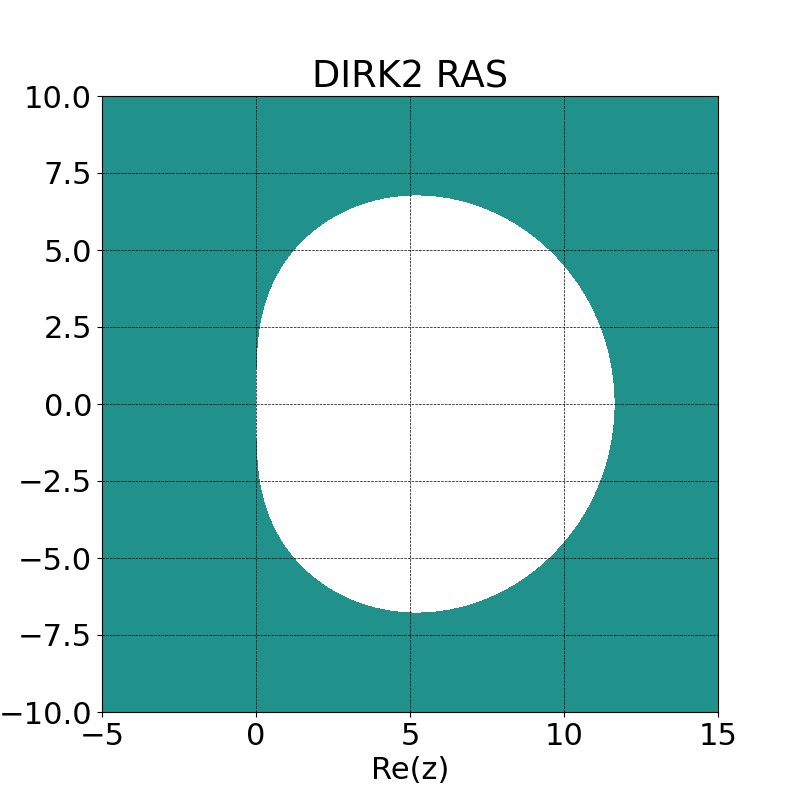
\includegraphics[scale=.3]{hw3 dirk2 RAS}
\end{center}
\sep



\tbf{Problem 2.} From the Butcher array,
$$A = \m{\gamma & 0 \\ 1-2\gamma & \gamma},
b = \m{1/2 \\ 1/2},
c = \m{\gamma \\ 1-\gamma}$$

\begin{enumerate}
	
\item \pf Check the 1st order accuracy condition.
$$\sum_{l=1}^2 b_l = \frac12 + \frac12 = 1$$
Check the 2nd order accuracy condition.
$$\sum_{l=1}^2 b_lc_l = \frac12\gamma+ \frac12(1-\gamma) = \frac12(\gamma+1-\gamma) = \frac12$$

\item \pf Check the 3rd order accuracy conditions.
$$\sum_{p,q,r} b_pa_{pq}a_{pr} = \frac12[\gamma^2+2\gamma\cdot0+0^2] + \frac12[(1-2\gamma)^2+2(1-2\gamma)\gamma+\gamma^2]$$
The quantity in the second bracket is
$$(1-2\gamma)^2+2(1-2\gamma)\gamma+\gamma^2 = 1+4\gamma^2-4\gamma+2\gamma-4\gamma^2+\gamma^2
= \gamma^2-2\gamma+1
= (\gamma-1)^2$$
giving
$$\sum_{p,q,r} b_pa_{pq}a_{pr} = \frac12[\gamma^2+\gamma^2-2\gamma+1] = \gamma^2-\gamma+\frac12$$
We find
$$\gamma^2 = \frac12+ \frac3{36} + 2\frac{3^{1/2}}{12}
= \frac1{12}[3+1+2\cdot 3^{1/2}]
= \frac1{12}[4+2\cdot 3^{1/2}]
= \frac16[2+3^{1/2}]$$
so finally,
$$\sum_{p,q,r} b_pa_{pq}a_{pr} = \frac16[2+3^{1/2}-3-3^{1/2}+3] = \frac13$$

\item First find the stability function $R(z)$.
$$I - zA = \m{1-\gamma z & 0 \\ -(1-2\gamma)z & 1-\gamma z}
\imp D := \det(I-zA) = (1-\gamma z)^2 = \gamma^2z^2 - 2\gamma z+1$$
$$\imp (I-zA)\inv = \frac1D\m{1-\gamma z & 0 \\ (1-2\gamma)z & 1-\gamma z}
\imp (I-zA)\inv 1_{s\times 1} = \frac1D\m{1-\gamma z \\ (1-2\gamma)z+1-\gamma z} = \frac1D\m{1-\gamma z \\ (1-3\gamma)z+1}$$
$$R(z) - 1 = zb^T(I-zA)\inv 1_{s\times 1} = \frac z{2D}\sbr{1-\gamma z+(1-3\gamma)z+1)}
= \frac z{2D}\sbr{(1-4\gamma)z+2}
= \frac12\frac{(1-4\gamma)z^2+2z}{\gamma^2z^2-2\gamma z+1}$$
We find $\gamma$ by imposing $\lim_{|z|\to\infty}R(z)=0$.
$$\lim_{|z|\to\infty}R(z)=0 \iff -1 = \frac12\lim_{|z|\to\infty}\frac{(1-4\gamma)z^2+2z}{\gamma^2z^2-2\gamma z+1}
\iff \lim_{|z|\to\infty}\frac{(1-4\gamma)z^2+2z}{\gamma^2z^2-2\gamma z+1} = -2
\iff \frac{1-4\gamma}{\gamma^2} = -2$$
$$\iff -2\gamma^2 = 1-4\gamma
\iff 2\gamma^2-4\gamma+1=0
\iff \gamma = \frac44 \pm \frac{(16-8)^{1/2}}4 = 1 \pm \frac{2\cdot 2^{1/2}}4 = 1\pm 2^{-1/2}$$
We check that the method for $\gamma=1\pm2^{-1/2}$ is A--stable, hence L--stable, by plotting the RASes and seeing that they contain the left half plane. Code in 3rd cell of:

\url{https://github.com/RokettoJanpu/Scientific-Computing-2/blob/main/hw3%20RAS.ipynb}

\begin{center}
\includegraphics[scale=.3]{hw3 dirk3 ras 1}
\includegraphics[scale=.3]{hw3 dirk3 ras 2}
\end{center}
	
\end{enumerate}

\end{document}